\section{Preliminaries}
\label{sec:Preliminaries}
Let $\F$ be the set of floating-point numbers. Given
\begin{itemize}
\item a cluster of $p$ \glspl{pe} indexed with a rank $i \in \{0, \ldots, p - 1\}$ and interconnected by a \gls{mpi}
\item $n_i$ floating-point numbers (elements) per \gls{pe} ($N := \sum_{i=0}^{p-1} n_i$ in total)
\item a not necessarily associative binary operation $\circ: \F \times \F \rightarrow \F$
\end{itemize}
we want to reduce all numbers by means of $\circ$ so that the end result is bitwise-reproducible.
A reduction algorithm is called bitwise-reproducible if multiple executions over the same set of numbers with a variable
number of \glspl{pe} produces bit-per-bit the exact same results.


\section{Related Work}
\label{sec:RelatedWork}

\subsection{Sequential left-to-right reduction}
\label{sec:SequentialLeftToRightReduction}


A naive approach to solving above problem is to gather all elements on a single PE and then apply the reduction operation strictly from left to right:

\begin{equation}
x_0 \circ x_1 \circ x_2 \circ \ldots  \circ x_{N-1} = ((x_0 \circ x_1) \circ x_2) \circ \ldots
\end{equation}

While simple in implementation, this approach suffers from one major drawback:
It does not benefit from any parallelization whatsoever.
Through the communication overhead, performance decreases with an increasing number of \glspl{pe}.


\subsection{Reproducible Accumulators}
\label{sec:Reproducible Accumulators}
For floating-point summation in particular, Ahrens et al.\ have developed an algorithm that uses a 6-word accumulator
to avoid unpredictable rounding errors \cite{ahrens_algorithms_2020}. After a read-only pass over the input data,
the summation can occur in parallel in no particular order and still produces bitwise identical results.
This requires around $9N$ floating-point operations and $3N$ bitwise operations.
The Reproducible Basic Linear Algebra Subprograms (ReproBLAS) software package implements this algorithm and
exposes a user-friendly API.\@

Naturally, this approach is not suitable for general reduction operations, since it depends on specific properties of floating-point numbers as specified in the IEEE 754 standard \cite{noauthor_ieee_nodate-1}.


\subsection{Reduction Tree}
\label{sec:ReductionTree}

\begin{figure}[H]
\centering
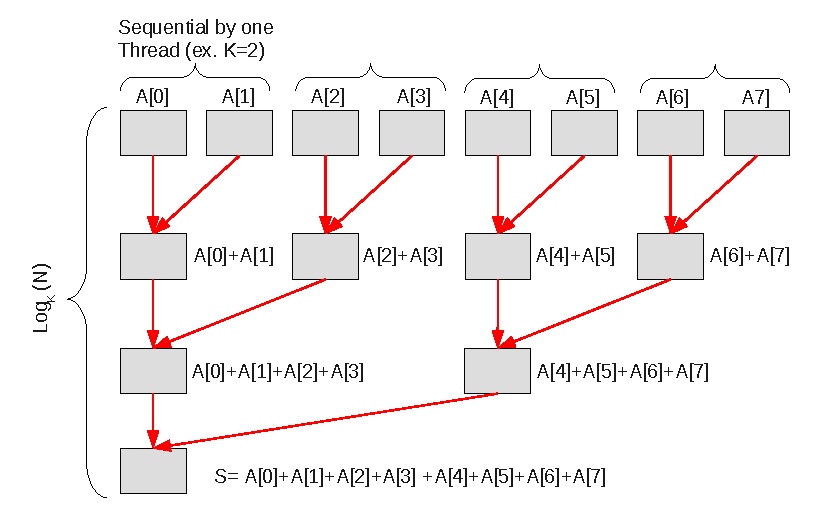
\includegraphics[scale=0.7]{figures/villa_et_al_reduction_tree.pdf}
\caption{General reduction tree (figure from Villa et al. \cite{villa_effects_2009})}
\label{fig:villa_reduction_tree}
\end{figure}


Villa et al.\ have utilized a $K$-ary tree structure on a Cray XMT system to sum floating-point numbers reproducibly \cite{villa_effects_2009}.
Figure \ref{fig:villa_reduction_tree} gives a schematic overview of the calculation order. Each leaf node has a single summand assigned to it
and each inner node sums up its up to $K$ child nodes. The algorithm then feeds the computed subtotal as input to the next layer of inner nodes.
$\log_K (N)$ levels of summations suffice to reduce all input numbers into a single value. Because the summation order only depends on the total number
of summands $N$ and the constant $K$, it should be reproducible across differently sized clusters.

The original source code is not available even after contacting the authors however, therefore the exact inner workings of this algorithm are
subject to speculation only.